\documentclass{beamer}
\usepackage[utf8]{inputenc}

\usetheme{Madrid}
\usecolortheme{default}
\useinnertheme{circles}

\definecolor{Logo1}{rgb}{0.208, 0.2865, 0.373}
\definecolor{Logo2}{rgb}{0.000, 0.674, 0.863}

\setbeamercolor*{palette primary}{bg=Logo1, fg=white}
\setbeamercolor*{palette secondary}{bg=Logo2, fg=white}
\setbeamercolor*{palette tertiary}{bg=white, fg=Logo1}
\setbeamercolor*{palette quaternary}{bg=Logo1,fg=white}
\setbeamercolor{structure}{fg=Logo1} % itemize, enumerate, etc
\setbeamercolor{section in toc}{fg=Logo1} % TOC sections

\usepackage{graphicx,animate}
%------------------------------------------------------------
%This block of code defines the information to appear in the
%Title page
\title[Linear Algebra] %optional
{Orthogonality, and Something Interesting...}

\subtitle{Lecture 7}

\author[11910803@mail.sustech.edu.cn] % (optional)
{
    Zhang Ce
}

\institute[] % (optional)
{
    Department of Electrical and Electronic Engineering\\
    Southern University of Science and Technology
}

\date[2021.11.9] % (optional)
{2021.11.9}


%End of title page configuration block
%------------------------------------------------------------



%------------------------------------------------------------
%The next block of commands puts the table of contents at the
%beginning of each section and highlights the current section:

\AtBeginSection[]
{
\begin{frame}
    \frametitle{Table of Contents}
    \tableofcontents[currentsection]
\end{frame}
}
%------------------------------------------------------------


\begin{document}

%The next statement creates the title page.
\frame{\titlepage}


%---------------------------------------------------------
%This block of code is for the table of contents after
%the title page
\begin{frame}
\frametitle{Table of Contents}
\tableofcontents
\end{frame}
%---------------------------------------------------------
\section{Orthogonal Vectors and Subspaces}
\begin{frame}{Inner Product (Dot Product)}
Actually, you have learnt that in your senior high school...

\vspace{3pt}
If I give you 2 vectors $\left[ \begin{array}{c}
	1\\
	2\\
\end{array} \right] ,\left[ \begin{array}{c}
	3\\
	1\\
\end{array} \right]$, how to compute its inner products?

\begin{equation*}
    \left[ \begin{array}{c}
        1\\
        2\\
    \end{array} \right] \cdot \left[ \begin{array}{c}
        3\\
        1\\
    \end{array} \right] =1\times 3+2\times 1=5
\end{equation*}

Recall matrix multiplications, which rule for matrix multiplication is similar to this?

\begin{equation*}
    \left[ \begin{matrix}
        1&		2\\
    \end{matrix} \right] \left[ \begin{array}{c}
        3\\
        1\\
    \end{array} \right] =3+2=5
\end{equation*}

Therefore, for 2 vectors $u$ and $v$, the inner product is $u^Tv$.

\vspace{3pt}
Take a deeper look, the result $5$ shows us... Think in geometrical way!
\end{frame}

\begin{frame}{Inner Product (Dot Product)}
\begin{figure}
    \centering
    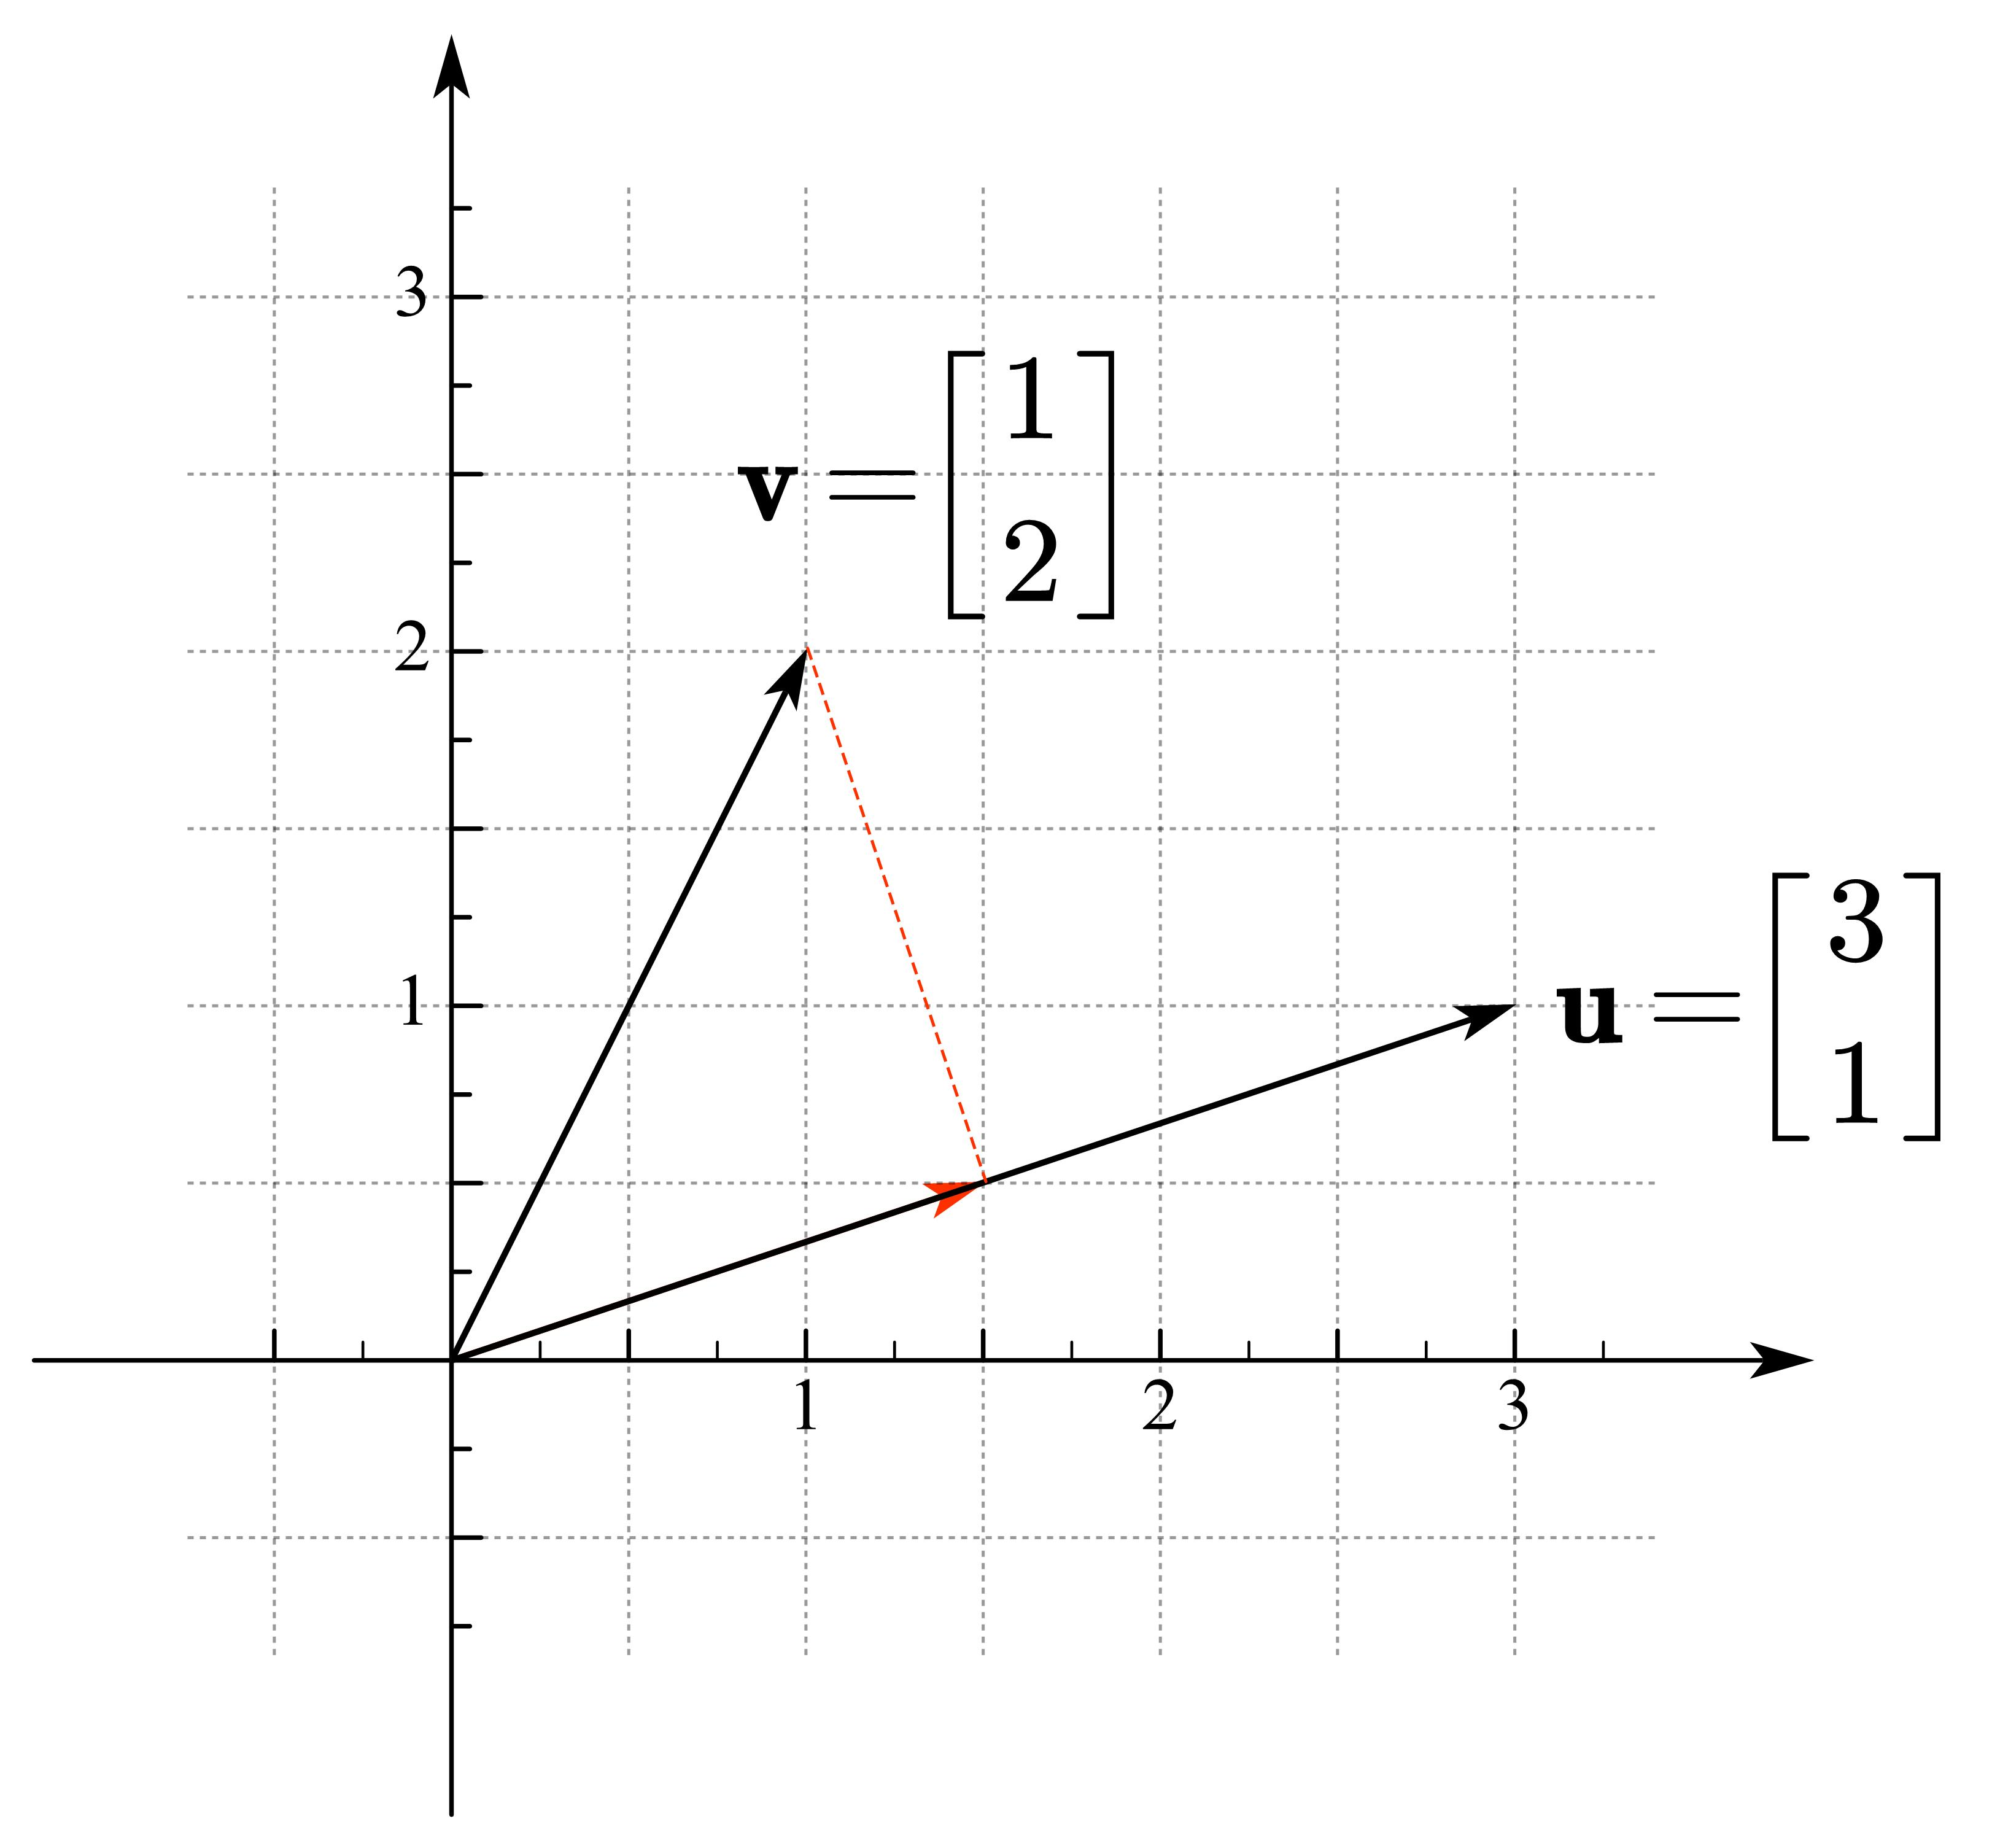
\includegraphics[width=0.47\textwidth]{ip.jpg}
\end{figure}

In my perspective, there inner product reflects their relevance. If the inner product can take the maximum or minimum value, then the vectors are dependent. While if the inner product is greater than zero, they point to the same direction, if it equals to zero, they have nothing to do with each other (perpendicular).
\end{frame}

\begin{frame}{Orthogonal Vectors and Subspaces}
Which value of inner product can let you realize that the vectors are perpendicular (\alert{orthogonal})?
\begin{equation*}
    u^Tv=0
\end{equation*}

Then we can further extend this definition to subspaces, if all the vectors in subspace $A$ are orthogonal to all the vectors in subspace $B$, then suspaces $A$ and $B$ are orthogonal.

\vspace{3pt}
One good question to ask: Is the blackboard plane perpendicular to the ground? But are they orthogonal?

\vspace{3pt}
Well, two orthogonal subspaces can only have the origin in common, and that is from the restriction of subspaces!
\end{frame}

\section{Projections onto Lines}
\begin{frame}{Projections}
Let's start from geometrical view. We want to find projection $\mathbf{p}$.
\begin{figure}
    \centering
    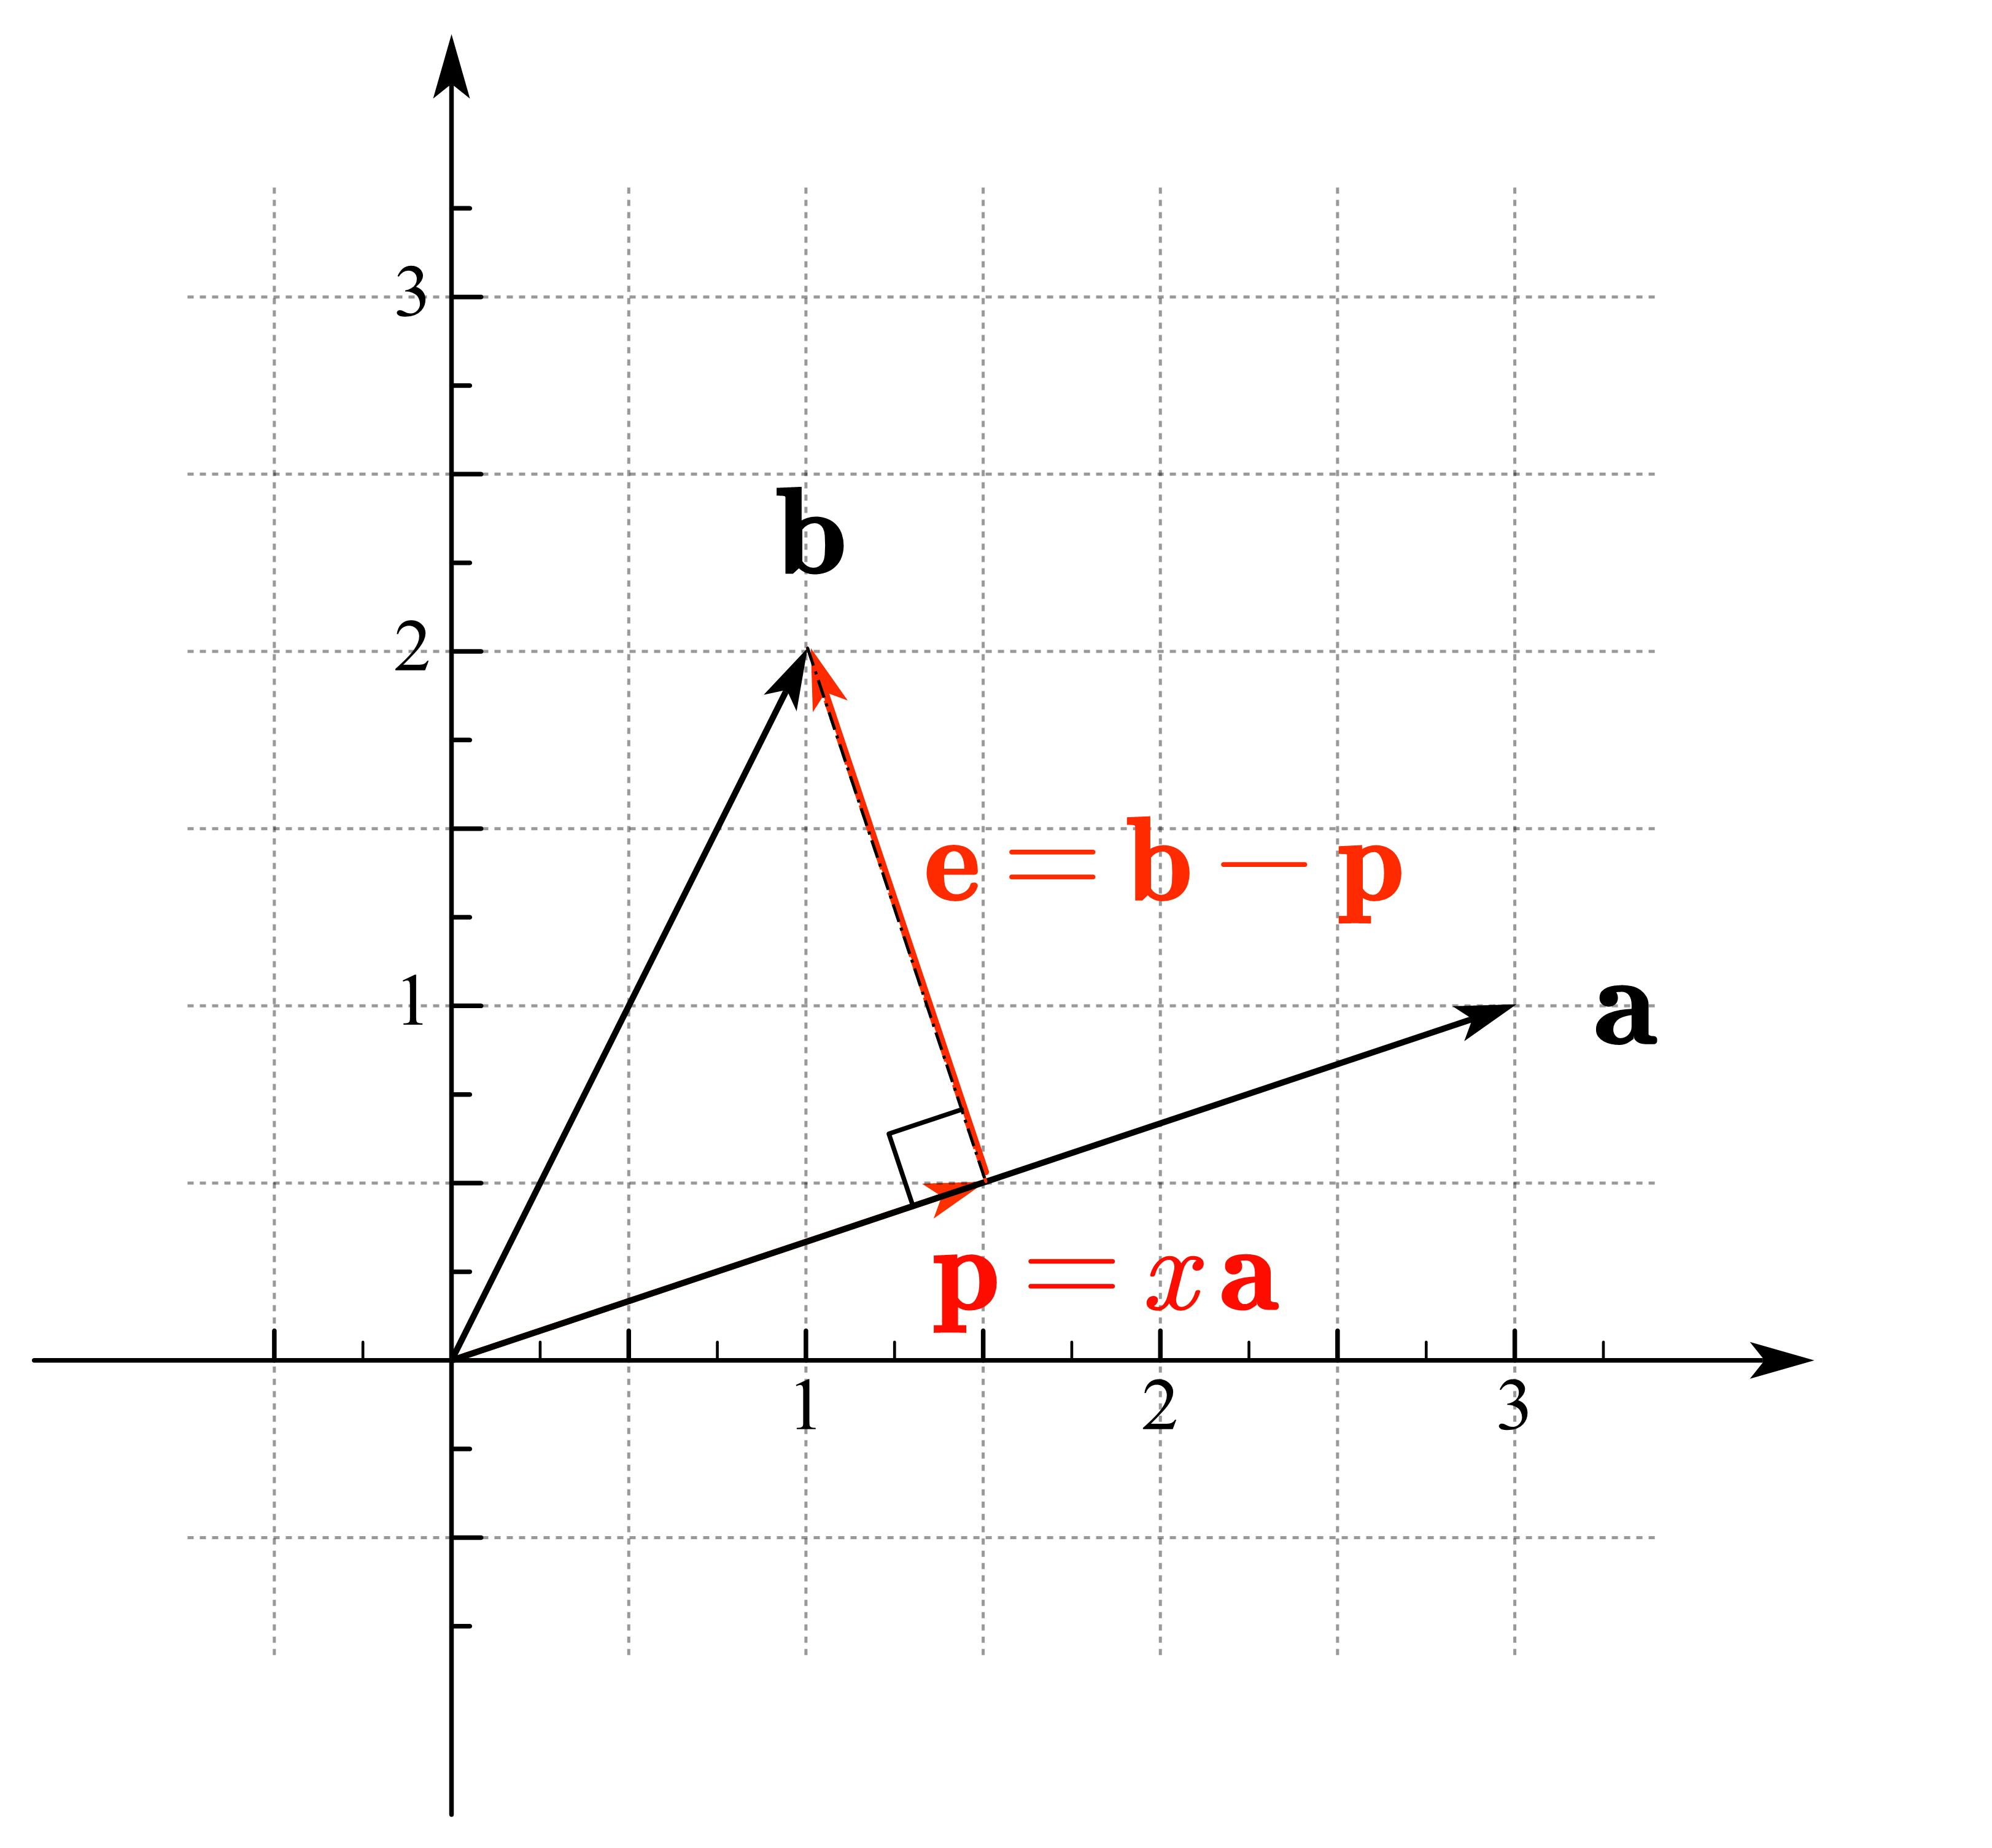
\includegraphics[width=0.45\textwidth]{projection.jpg}
\end{figure}

What can we get from that 90 degrees? Can we get an expression of $\mathbf{p}$?
\begin{equation*}
    \mathbf{a}^T\mathbf{e}=\mathbf{a}^T\left( \mathbf{b}-x\mathbf{a} \right) =0\Rightarrow x=\frac{\mathbf{a}^T\mathbf{b}}{\mathbf{a}^T\mathbf{a}}\Rightarrow \mathbf{p}=\mathbf{a}\frac{\mathbf{a}^T\mathbf{b}}{\mathbf{a}^T\mathbf{a}}
\end{equation*}
What if the length of vector $\mathbf{a}$ doubles? How about $\mathbf{b}$?
\end{frame}

\begin{frame}{Projection Matrix}
    \begin{equation*}
        \mathbf{a}^T\mathbf{e}=\mathbf{a}^T\left( \mathbf{b}-x\mathbf{a} \right) =0\Rightarrow x=\frac{\mathbf{a}^T\mathbf{b}}{\mathbf{a}^T\mathbf{a}}\Rightarrow \mathbf{p}=\mathbf{a}\frac{\mathbf{a}^T\mathbf{b}}{\mathbf{a}^T\mathbf{a}}
    \end{equation*}
Can you give a projection matirx that can project every vector $b$ onto the line where $a$ lies in?
\begin{equation*}
    \mathbf{p}=P\mathbf{b}\Rightarrow P=\frac{\mathbf{aa}^T}{\mathbf{a}^T\mathbf{a}}
\end{equation*}
That is the matrix for projection onto line $a$. Use your knowledge of previous knoledge, $\mathbf{aa}^T$ is a scalar, vector or matrix? What about $\mathbf{a}^T\mathbf{a}$?

\vspace{3pt}
Think in linear transformation, what is the rank of that matrix $P$, that is to ask the dimension of the output space (the column space).

\vspace{3pt}
Definitely 1, I can also get the column space is the line containing vector $\mathbf{a}$.

\vspace{3pt}
Some properties for projection matrix $P$?
\end{frame}

\section{Least Squares}
\begin{frame}{Motivation}
In Chapter 2, when we meet a linear equation system $Ax=b$, it may have no solutions. But we can find a solution that can minimize the error! In practice, if we have more equations than the variables, we may want to find the best approximation solution.

\vspace{3pt}
Take fitting as an example:
\begin{figure}
    \centering
    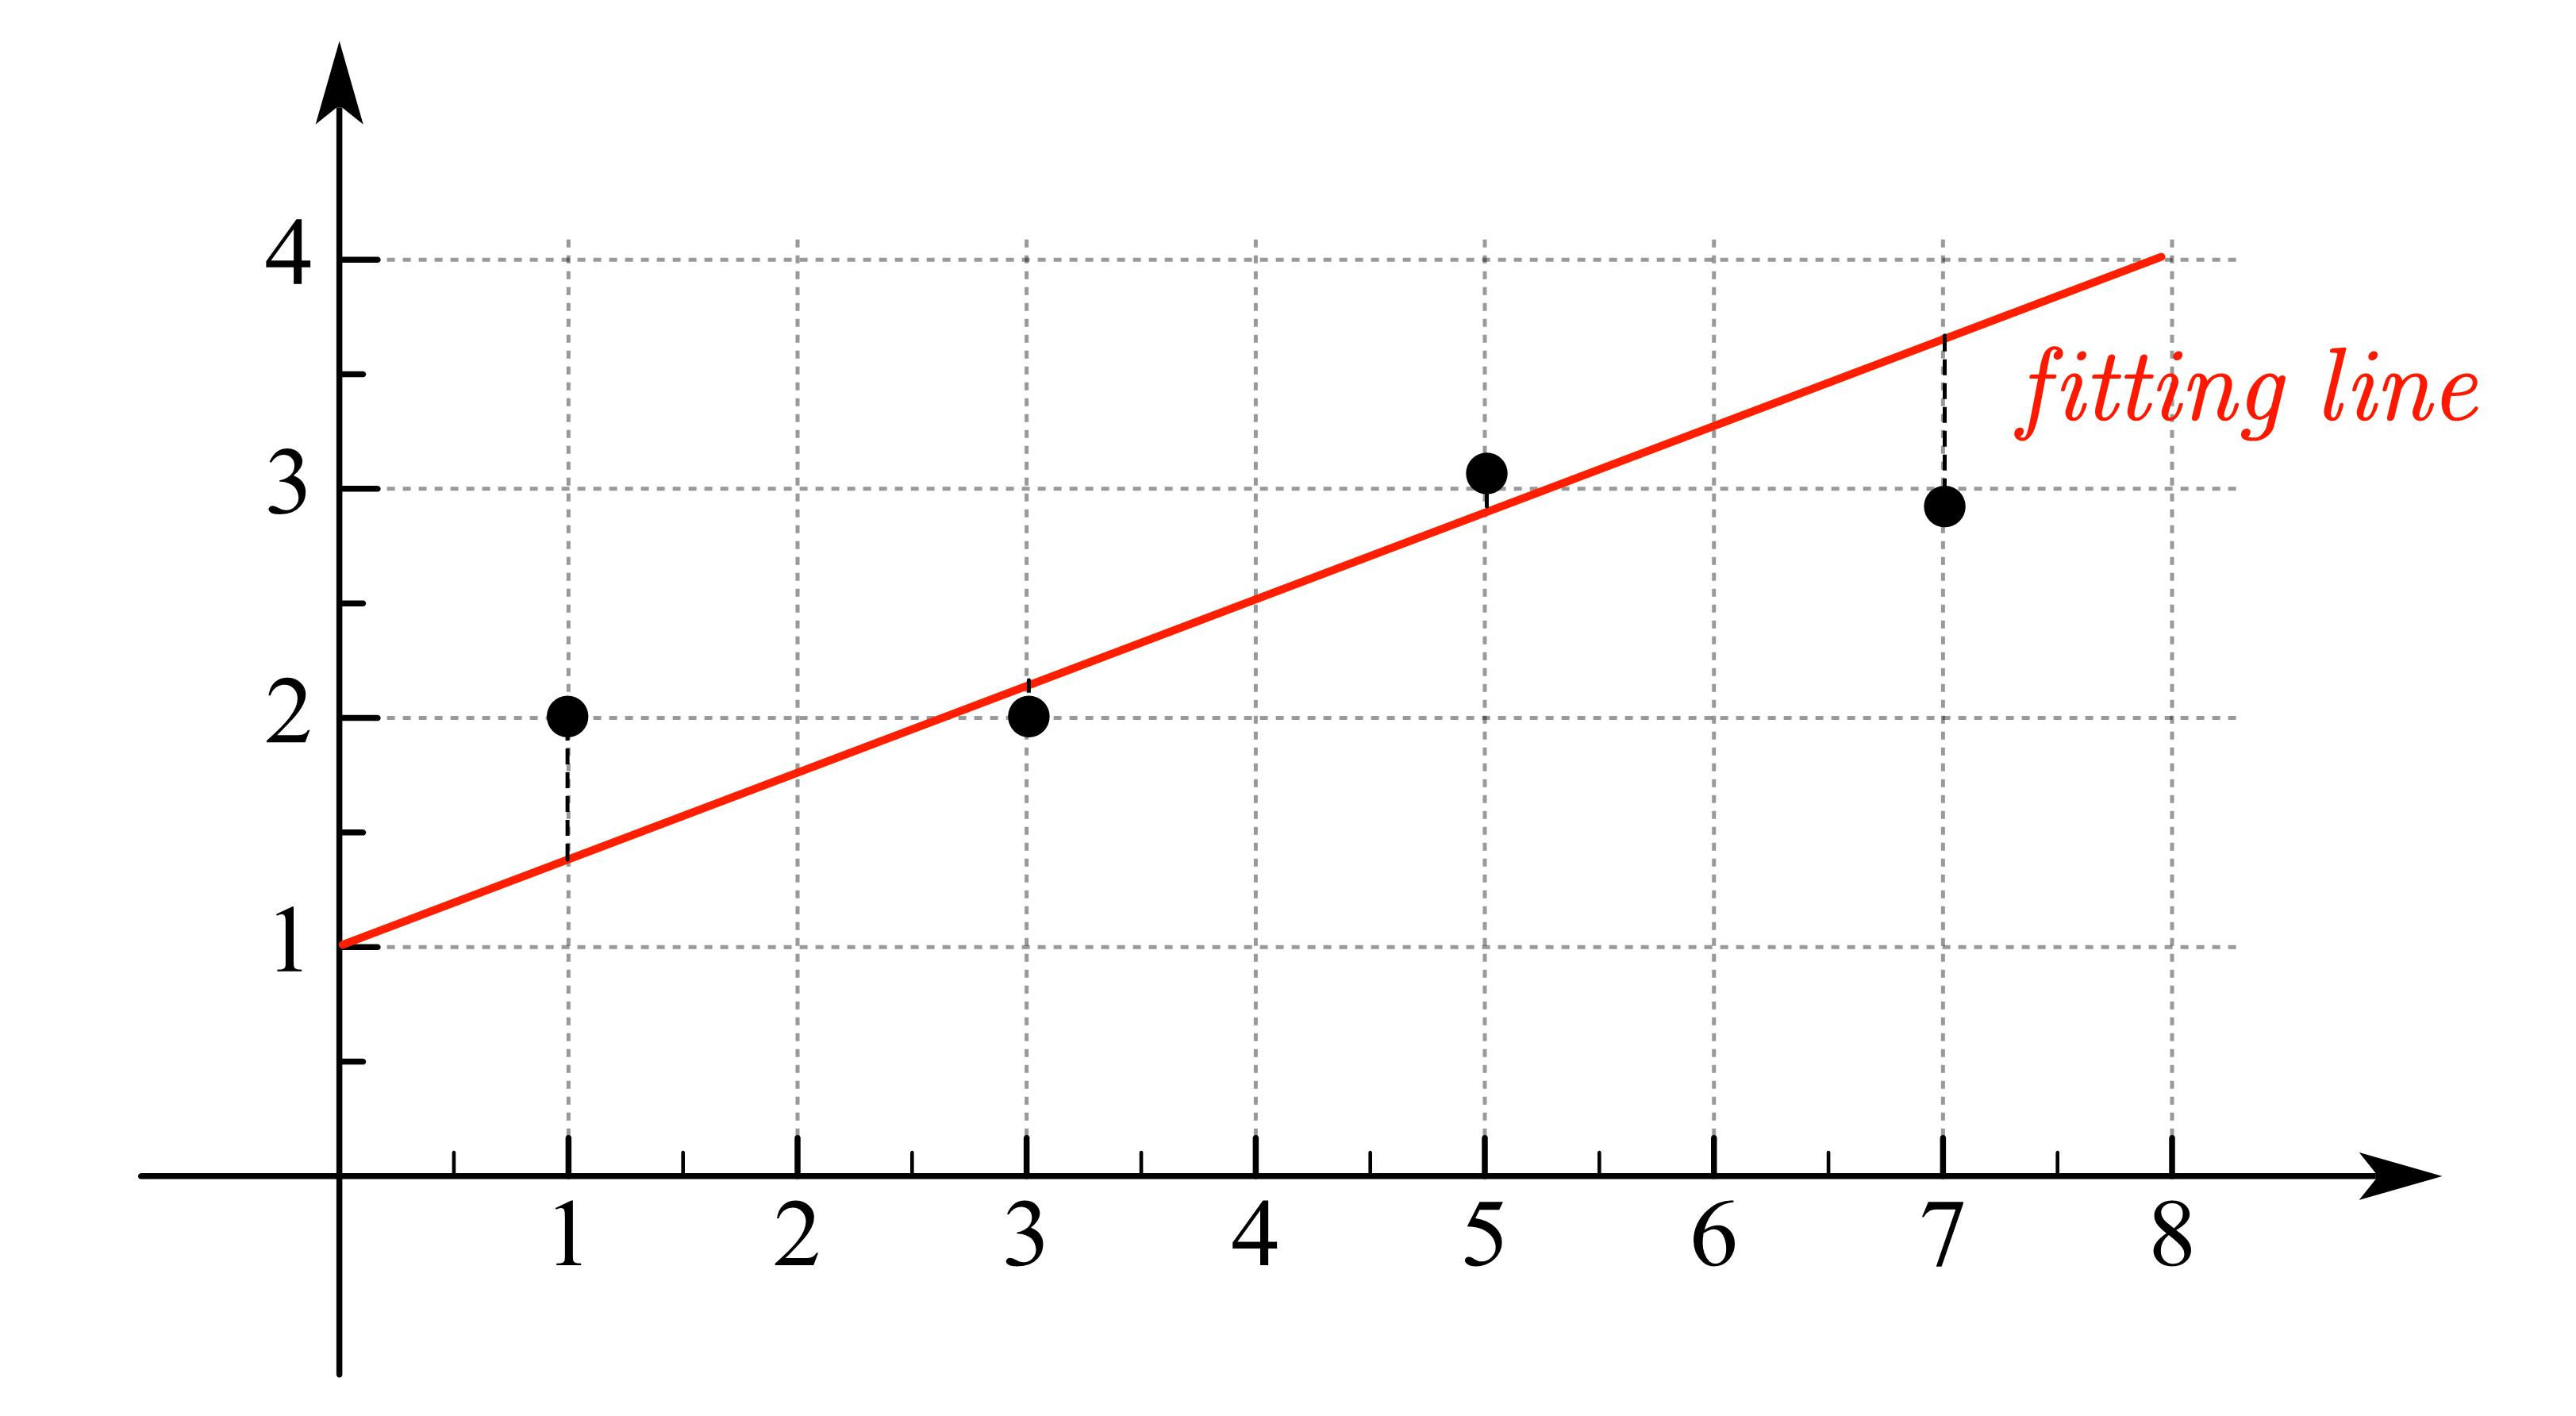
\includegraphics[width=0.62\textwidth]{fitting.jpg}
\end{figure}
We can't find a line to cover all the points, but we can find the line that minimizes the error.
\end{frame}

\begin{frame}{Motivation}
\vspace{3pt}
Take fitting as an example:
\begin{figure}
    \centering
    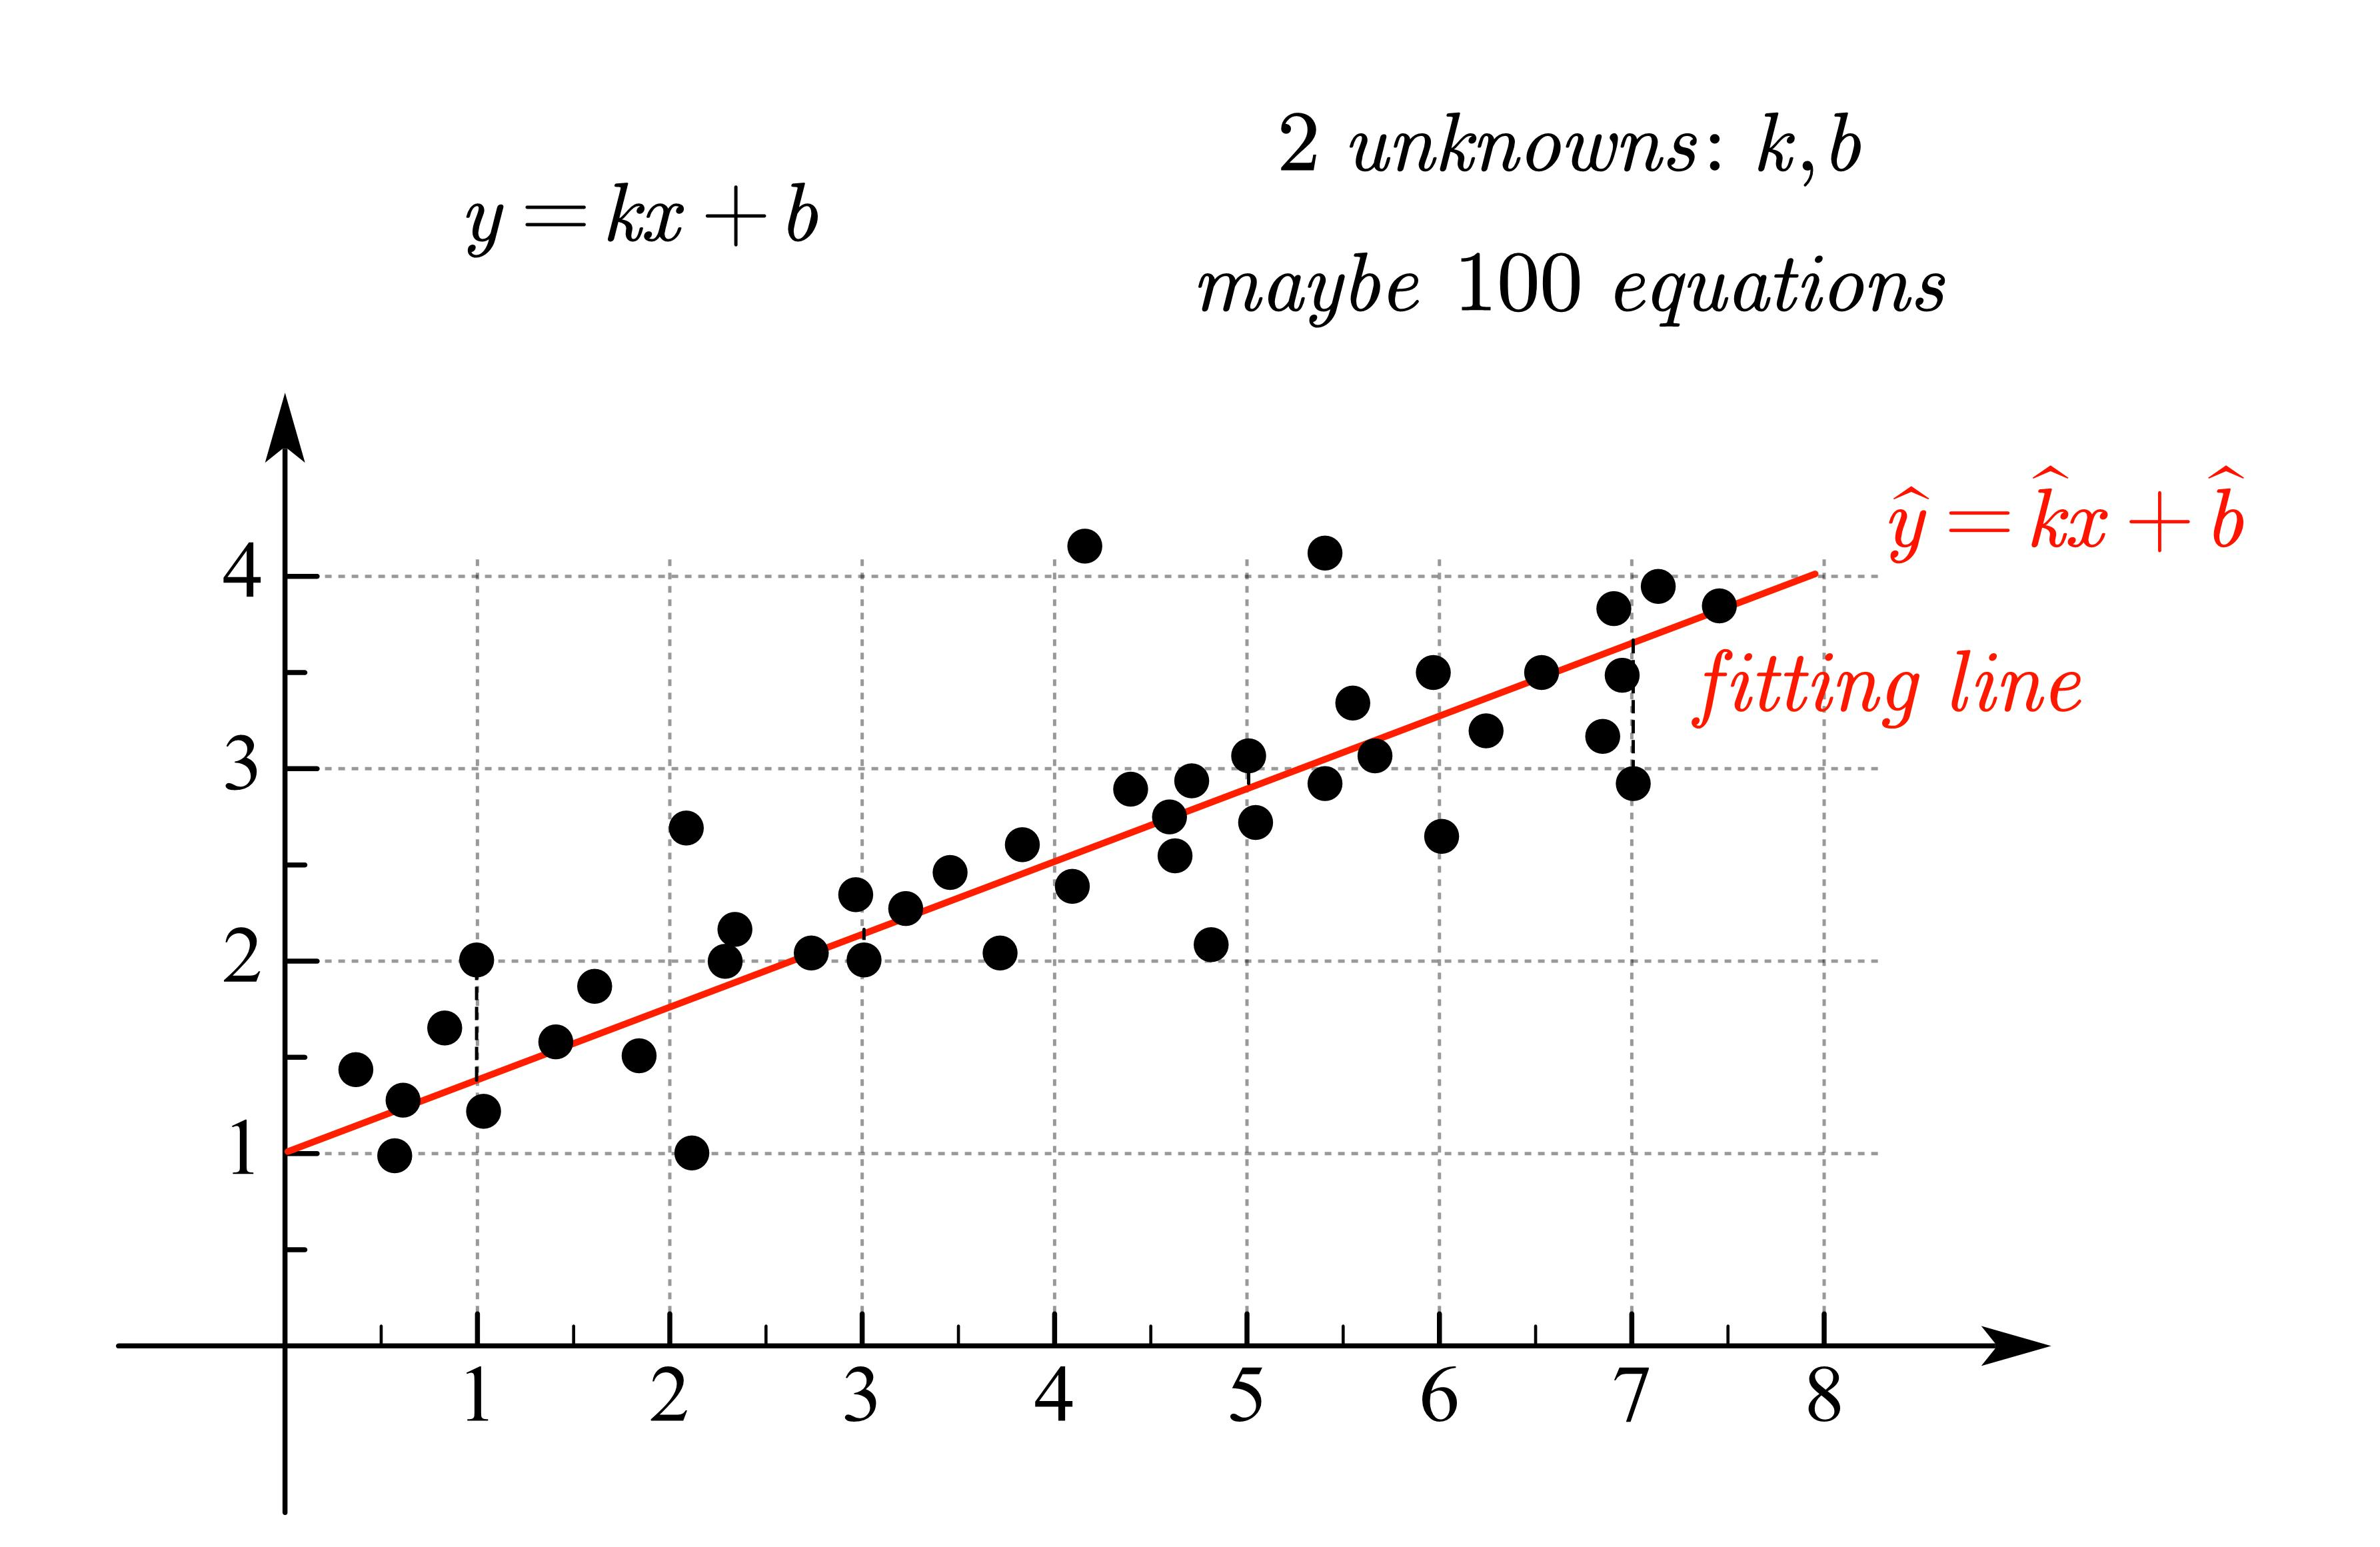
\includegraphics[width=0.75\textwidth]{fitting2.jpg}
\end{figure}

How to find the predicted line? The answer is: least-squares.
\end{frame}

\begin{frame}{Least-Squares}
The core is: find the solution for $Ax=p$ (A is the matrix with $a_1,a_2$ in columns) where $p$ is the projection on $C(A)$, which can definitely gives a unique solution.

\begin{figure}
    \centering
    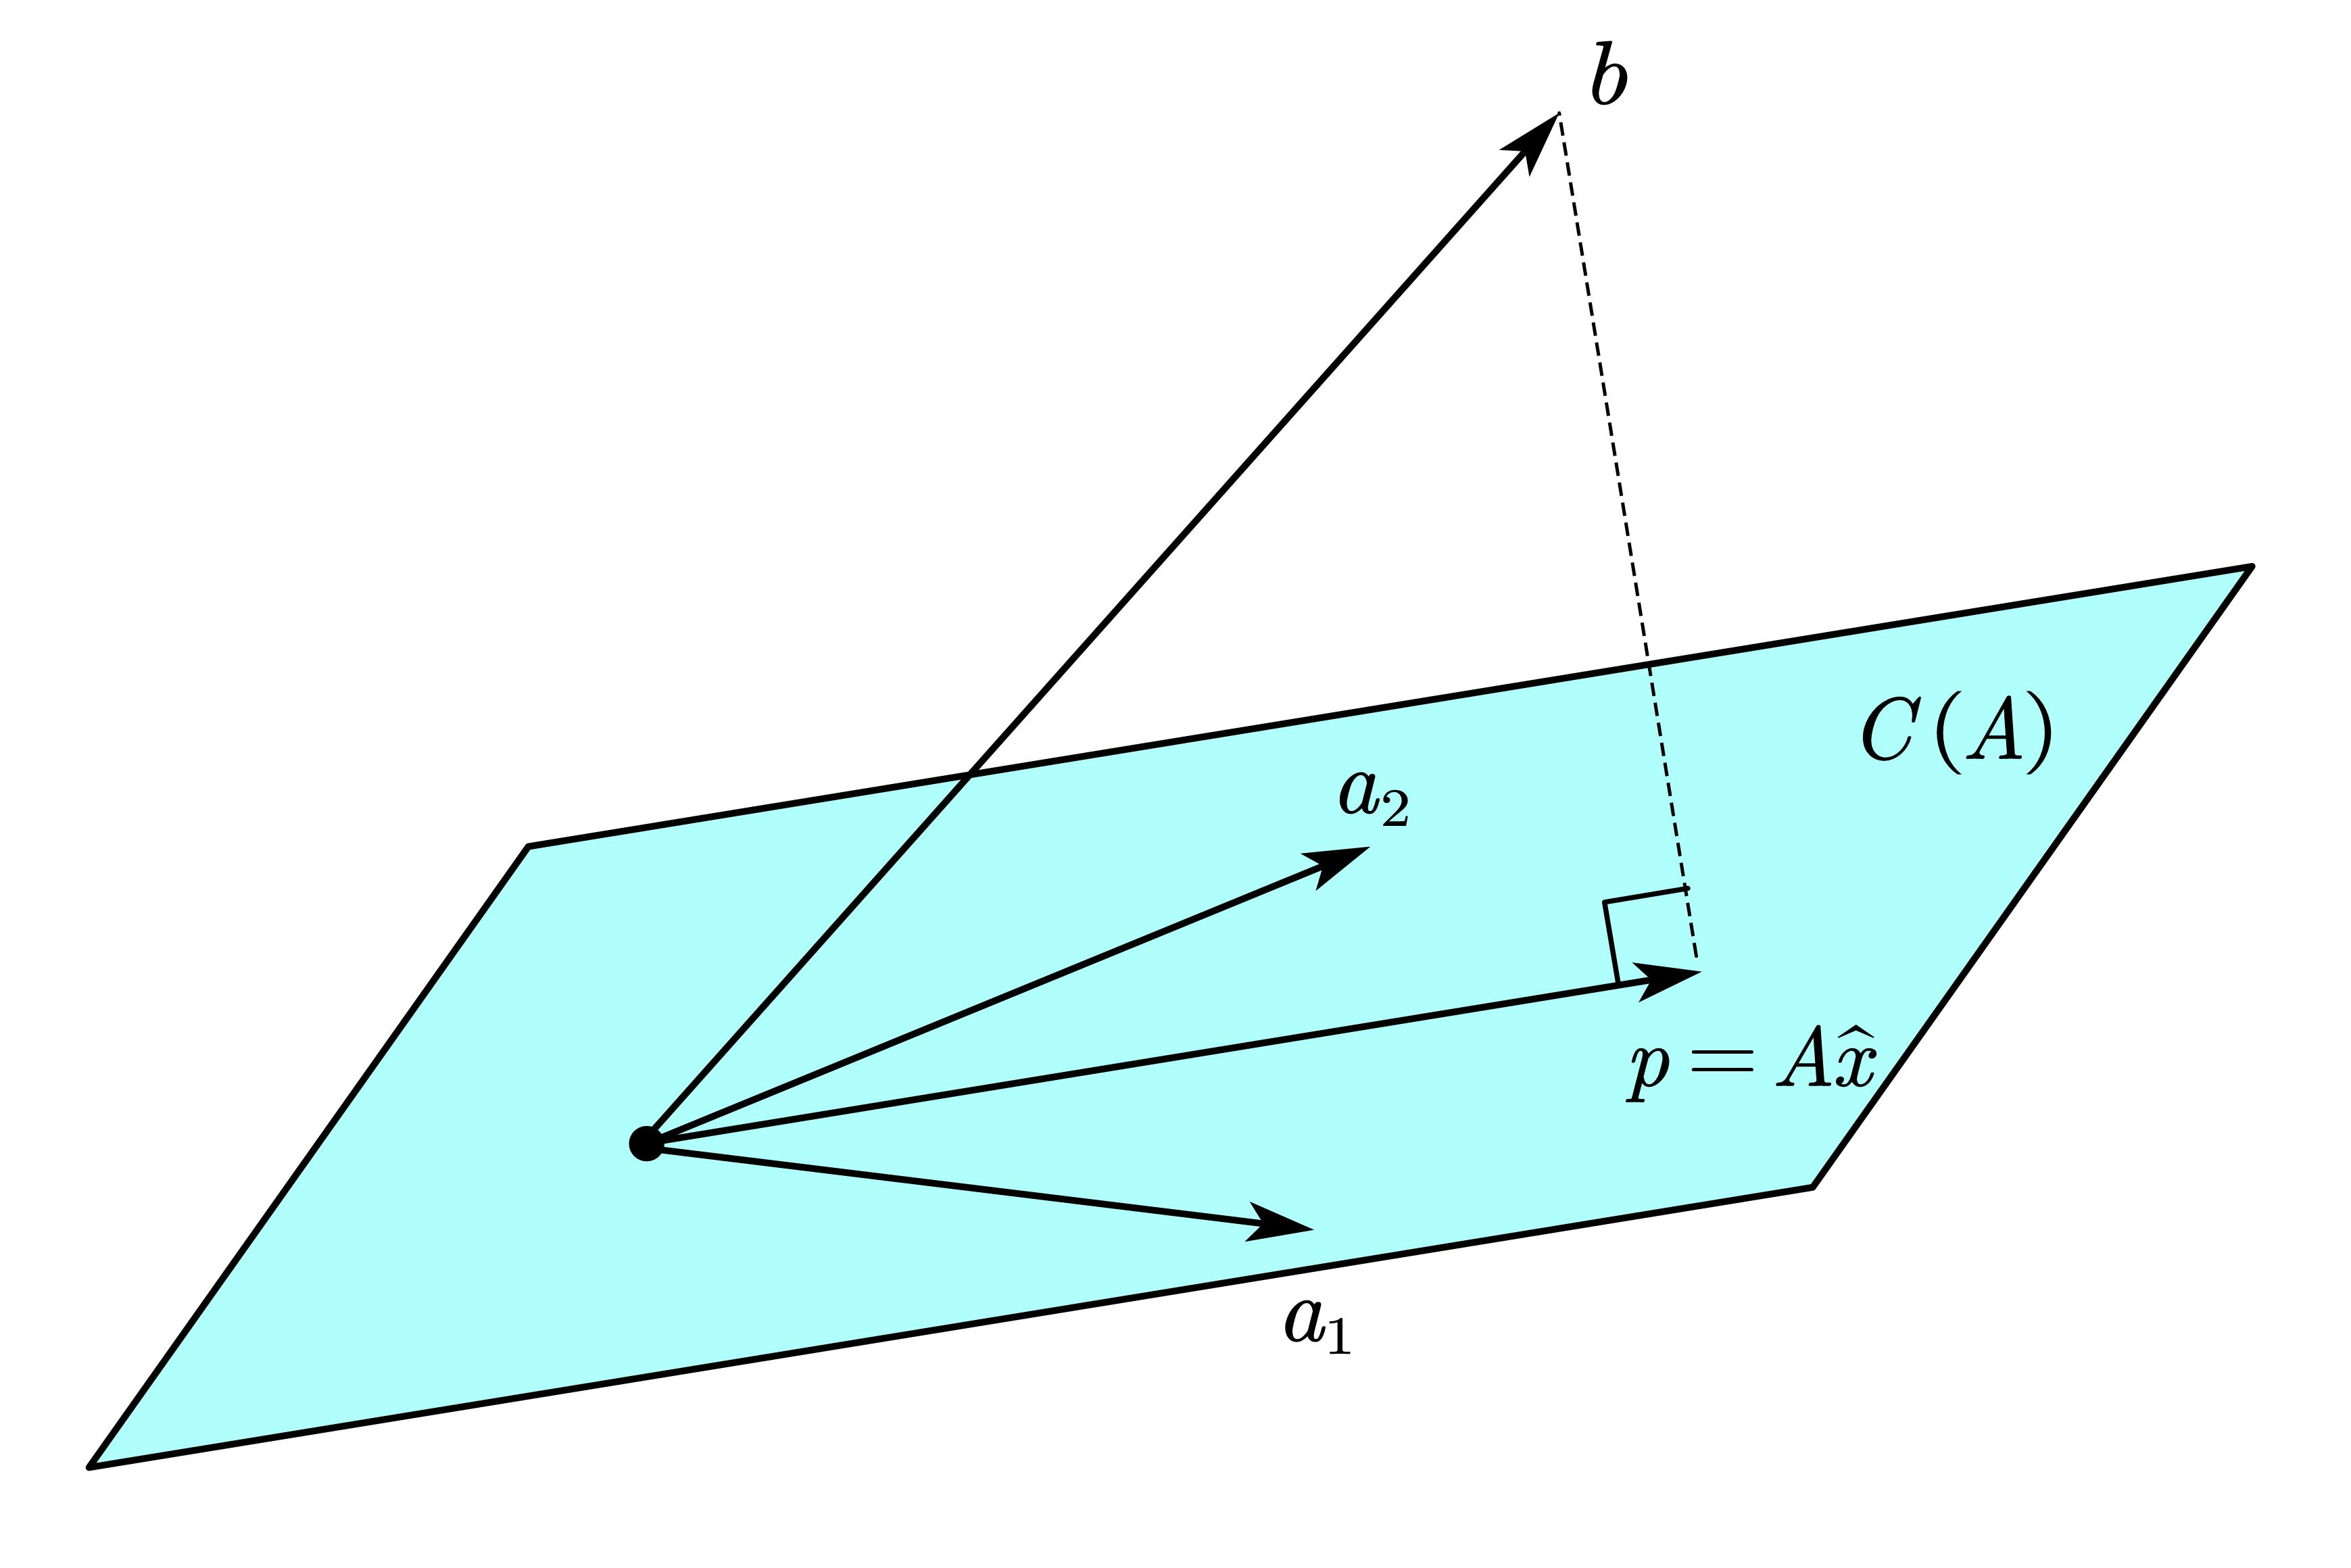
\includegraphics[width=0.5\textwidth]{ls.jpg}
\end{figure}
\begin{equation*}
    {a_1}^T\left( b-A\hat{x} \right) ={a_2}^T\left( b-A\hat{x} \right) =0
\end{equation*}

The error $e=b-p=b-A\hat{x}$ is in the nullspace of $A$, while the projection $p=A\hat{x}$ is in the column space of $A$!
\end{frame}

\begin{frame}{Least-Squares}
Well, we can simplify that equation...
    \begin{equation*}
        {a_1}^T\left( b-A\hat{x} \right) ={a_2}^T\left( b-A\hat{x} \right) =0
    \end{equation*}
\begin{equation*}
    \left[ \begin{array}{c}
        {a_1}^T\\
        {a_2}^T\\
    \end{array} \right] \left( b-A\hat{x} \right) =\left[ \begin{array}{c}
        0\\
        0\\
    \end{array} \right]
\end{equation*}
\begin{equation*}
    A^T\left( b-A\hat{x} \right) =0
\end{equation*}
\begin{equation*}
    A^TA\hat{x} =A^Tb
\end{equation*}

Now, can you tell me why $A^TA\hat{x} =A^Tb$ must be consistent? The reason behind: $Ax=p$ must have solutions.

\vspace{3pt}
Finally, we can get:
\begin{equation*}
    \hat{x} =(A^TA)^{-1}A^Tb
\end{equation*}

That is the least-squares solution, indicating how to combine the columns in $A$ can we get the nearest vector to $b$.
\end{frame}

\begin{frame}{Projection Matrices}
We have introduced projection matrices onto lines:
\begin{equation*}
    P=\frac{\mathbf{aa}^T}{\mathbf{a}^T\mathbf{a}}
\end{equation*}

\end{frame}

\end{document}